\documentclass[twocolumn,showpacs,preprintnumbers,amsmath,amssymb]{revtex4}
%\documentclass[preprint,showpacs,preprintnumbers,amsmath,amssymb]{revtex4}
% Additional packages needed for graphics, alignment and math fonts.

\usepackage{graphicx}% Enhanced capability for dealing with figures
\usepackage{dcolumn}% Align table columns on decimal point.
\usepackage{bm}% bold math.
\usepackage{amsmath}
\usepackage{tikz}
\usepackage{quantikz}
% The \begin{document} command sets the start of the RevTeX commands.
	
	\begin{document}
		
		\title{A quantum algorithm for the Bottleneck Travelling Salesman Problem}
		
		\author{Raveel Tejani}
		\email{raveel@student.ubc.ca}
		\affiliation{Department of Physics and Astronomy, University of British
			Columbia \\
			6224 Agricultural Road, Vancouver, British Columbia, V6T 1Z1, Canada}
		
		\date{\today}
		
		\begin{abstract}
			%statement of what will be accomplished, the methods that will be used and
			%the potential significance.  Many of you have already sent me a description
			%of your project that can be used as the basis for this.  I will only accept
			%\LaTeX\ complied files in pdf format (and we're going to specifically use
			%revtex, the style for Physical Review). They must be uploaded by midnight
			%before the oral presentation is scheduled.  Make sure your supervisor has
			%a chance to read it over before you submit it.
			
			The Bottleneck Travelling Salesman Problem (BTSP) stands as an NP-Hard optimization problem, suggesting a lack of solutions in polynomial time. With a complexity of $(N-1)!$ for $N$ cities, the need for a more efficient solution becomes evident. In response, we propose the development of an algorithm rooted in quantum phase estimation and Grover's algorithm, aiming to provide a solution within the improved time frame of $\sqrt{(N-1)!}$. To validate the efficacy of our proposed quantum algorithm, testing will be conducted on simulators and potentially real quantum hardware. Subsequent to the experimental phase and implementation of enhancements, we will present our findings and insights gained. The research doesn't just aim to offer a quantum-powered solution to the BTSP but also adds to the conversation about how quantum algorithms can change how we solve tough optimization problems.
			
		\end{abstract}
		
		\maketitle
		
		% The first section of the paper.
		
		\section{Motivation}
		
		
		Continuous advancements in quantum computing have opened new ways to solve complex computational problems that were previously considered intractable using classical methods. Well known examples of these advancements include Shor's \cite{Shor} and Grover's \cite{grover1996fast} algorithm for factoring and unstructured search respectively. The Bottleneck Traveling Salesman Problem (BTSP) serves as a challenging optimization problem in the field of logistics and operations research. Its practical applications range from optimizing vehicle routes to circuit design. Consequently, achieving an efficient solution is highly sought after. However, the BTSP is classified as an NP-hard problem, indicating it is at least as difficult as the hardest problems in the NP class. For reference, an NP problem must satisfy two conditions: no known solution in polynomial time, and a solution can be verified in polynomial time. An NP-hard problem does not need to satisfy the verification condition. To address this problem, many heuristic approaches are explored \cite{heuristicthesis}\cite{heuristic}. However, inherent to such methods is a trade-off between precision and efficiency.
		
		We embark on a journey at the intersection of quantum computing and optimization by introducing a quantum algorithm tailored to address the BTSP. It requires finding the shortest closed tour through a set of cities while minimizing the largest cost, the "bottleneck", along any route. Its computational complexity grows exponentially with the number of cities, rendering classical solutions impractical for large-scale instances. Our approach is to capitalize on the inherent quantum parallelism, as well as the unique feature of phase encoding in quantum computing. By exploiting these phenomena, we aim to encode and manipulate the costs associated with various routes efficiently. Additionally, the utilization of Grover's search algorithm as a central component of our quantum approach significantly expedites the search for the optimal solution.  Quantum searching, in general, may be useful for obtaining solutions faster for problems belonging to the complexity class NP \cite{nielsen00}. In this proposal, our primary objective is to shed light on the theoretical foundation of the quantum algorithm, its potential computational advantages over classical methods. Through this research, we aim to work towards a clear understanding of these aspects. The following sections will detail the BTSP, Grover's algorithm, quantum phase estimation and their respective significance and complexity. 
		
		
		\section{Theory}
		
		\subsection{Bottleneck Travelling Salesman Problem}
		
		\begin{figure}[!h]
			\centering
			\includegraphics[trim={0 0 21.9cm 0},clip, width=0.7 \linewidth]{"graphics/4-city"}
			\caption{An undirected weighted graph represention of a  symmetric 4-city system.  The vertices represent cities and the edge weights represent the cost of travel. }
			\label{fig:4-city-graphic}
		\end{figure}		
		
		The BTSP can be represented as a graph problem.  We start with a graph, whose vertices are labelled A through D, representing a 4-city system. We define movement from one vertex to another as a walk, done through the edges connecting our vertices. We are interested in a particular walk known as a Hamiltonian cycle that contains every vertex exactly once before returning to the start. Our graph also includes edge weights, we define as $ \gamma_i $.
		The BTSP is to find the Hamiltonian cycle in a graph, where the largest edge weight (bottleneck) is minimized. This is distinct from the Travelling Salesman Problem (TSP) where the combined edge weights in a given cycle is minimized. The total possible Hamiltonian cycles is given by $(N-1)!$, where N is the number of nodes. We present a symmetric case in FIG .\ref{fig:4-city-graphic},  $N_k \rightarrow N_{k+1} = N_{k+1} \rightarrow N_{k} = \gamma_i$. Thus the total possible cycles is  $(N-1)!/2$.  It is important to note that a solution to either BTSP or TSP is not unique. BTSP solutions also do not necessarily equate to the TSP solutions. We can illustrate an example below. Consider all the Hamiltonian cycles for a symmetric 4-city system:
		
		\begin{center}
		$ A \rightarrow B \rightarrow C \rightarrow D \rightarrow A $
		
		$ A \rightarrow B \rightarrow D \rightarrow C \rightarrow A $ 
		
		$ A \rightarrow C \rightarrow B \rightarrow D \rightarrow A $
	    \end{center}
		
		Assigning some arbitrary weights, we can see the total costs of the cycles below. The first cycle is the solution to BTSP as its largest edge weight at $5$ is the smallest among all three. The last cycle is a solution to the TSP as its combined edge weight is the smallest.
		\begin{center}
		$\gamma_1 + \gamma_4 + \gamma_5 + \gamma_3 = 4 + 4 + 5 + 4 = 17$
		
		$ \gamma_1 + \gamma_6 + \gamma_5 + \gamma_2 = 4 + 6 + 5 + 2 = 17$
		
		$  \gamma_2 + \gamma_4 + \gamma_6 + \gamma_3 = 2 + 4 + 6 + 4 = 16$
		\end{center}
		

		By simply changing the weight of $\gamma_6$ to $5$, we can illustrate all cycles are solutions to the BTSP. 
		
		\begin{center}

			$\gamma_1 + \gamma_4 + \gamma_5 + \gamma_3 = 4 + 4 + 5 + 4 = 17$
			
			$ \gamma_1 + \gamma_6 + \gamma_5 + \gamma_2 = 4 + 5 + 5 + 2 = 16$
			
			$  \gamma_2 + \gamma_4 + \gamma_6 + \gamma_3 = 2 + 4 + 5 + 4 = 15$
		\end{center}
		
		The computational complexity of the BTSP is known to be NP-hard. Implying there is no algorithm for a solution in polynomial time. A brute-force approach would imply that we can run an algorithm in $O((N-1)!)$ time.
		\subsection{Grover's Search Algorithm}
		
		\begin{figure}[!h]
			\centering
			\includegraphics[trim={4.5cm 26cm 15cm 0},clip, width=0.99 \linewidth]{"graphics/grov_circ"}
			\caption{A concise quantum circuit representation of Grover's search algorithm applied to an n-qubit system. The Hadamard $H^{\otimes n }$ gate creates a uniform superposition over all possible states $N$ ($2^n$). The $U_w$ gate marks our goal state. The $U_s$ gate amplifies the amplitude of our goal state. the $r$ exponent, refers to the number of iterations needed to maximize the amplitude. The approximate number is $\sqrt{N}$ times.}
			\label{fig:grovercircuit}
		\end{figure}
		
		In 1996, Lov Grover proposed a quantum algorithm for unstructured database search, where an $N$ sized list could be searched in $\sqrt{N}$ time \cite{grover1996fast}. This speed up can be realized for sufficiently large databases, but does not provide the exponential speedup promised by other quantum algorithms such as Shor's \cite{Shor}. We can refer to FIG. \ref{fig:grovercircuit}, to see the quantum circuit representation. We will use the geometric representation of the algorithm shown in FIG. \ref{fig:grovergeometric}, to aid our understanding of the algorithm.  
		
		
		\begin{figure}[!h]
			\centering
			\includegraphics[trim={0 7.5cm 0 0},clip, width=0.99\linewidth]{"graphics/grov_geom"}
			\caption{Geometric reprentation of Grover's algorithm.  a) An iteration performed on an n-qubit system.  Starting from the uniform superposition $|s\rangle$, we perform a reflection over the orthogonal states of $|w\rangle$ with $U_w$. Then we perform a reflection over the superposition state $|s\rangle$ with $U_s$. we can see our new state $|x\rangle = U_sU_w|s\rangle$ is closer to the goal state $|w\rangle$. A new iteration would imply reflecting again over $|w_\perp\rangle$ and then reflecting back over $|x\rangle$. b) An iteration performed on a 2-qubit system. Only one iteration is required to hit any goal state $|w\rangle$. }
			\label{fig:grovergeometric}
		\end{figure}
		
		Lets walk through one iteration of Grover's algorithm. Most quantum circuits are initialized at $|0\rangle$, then we apply the $H$ gate, this results in a uniform superposition:
		
		\begin{equation}
		 |s\rangle = H^{\otimes n} |0^{\otimes n} \rangle = \frac{1}{\sqrt{2^n}} \sum_{x\in\{0,1\}^n} |x\rangle
		\end{equation}
	%	$$ |s\rangle_2 = H^{\otimes 2} |0 \rangle = \frac{1}{2} (|00\rangle + |01\rangle + |10\rangle + |11\rangle)$$
		
		The orthogonal states to our goal state can be represented as the sum of all states not containing $|w\rangle$
		
		$$ |w_\perp\rangle=  \frac{1}{\sqrt{2^n -1}} \sum_{x\in\{0,1\}^n}^{x \neq w} |x\rangle$$
		
		From here we apply the $U_w$ gate, for our reflection over the orthogonal states. This can be thought of flipping the sign on state $|w\rangle$ contained within $|s\rangle$. We can see the visual representation in FIG. \ref{fig:grovergeometric}. We then perform a similar reflection over the original state $|s\rangle$ :
		
		$$ U_w|s \rangle	=  (\mathbb {I} - 2|w \rangle \langle w|) |s \rangle = |s'\rangle$$
		$$ U_s|s' \rangle	=  (2|s \rangle \langle s| - \mathbb {I}) |s' \rangle = |s''\rangle$$
		
		Our $|s''\rangle$ is now closer to our goal state $|w\rangle$.  If we want to maximize our probability of measuring  $|w\rangle$, we will need to perform a number of iterations ($r$). For sufficiently large number of states, $N = 2^n$, we can make a few approximations to calculate $r$.
		\begin{equation}
			\langle w | s \rangle = \frac{1}{\sqrt{N}} = \sin \frac{\theta}{2} \approx \frac{\theta}{2}
		\end{equation}
		
		
		$$P(w) = |\langle w | s \rangle|^2 = \frac{1}{N} = \sin^2 \frac{\theta}{2} $$
		
		$$P(w) = |\langle w |(U_sU_w)^r |s \rangle|^2 = \frac{1}{N} = \sin^2 \left(\theta\left(\frac{1}{2} + r\right)\right) $$
		
		To maximize the probability we need P(w) = 1, so we can set the inside of the sine function to $\pi/2$:
		$$ \theta \left(\frac{1}{2} + r \right) = \frac{\pi}{2}$$
		
		\begin{equation}
			r = \frac{\pi}{2\theta} + \frac{1}{2} \approx \frac{\pi}{2\theta}
		\end{equation}
		
		Using eqn. 2 to substitute $\theta$ in eqn. 3, we can get an approximate result for r:
		
		\begin{equation}
			r \approx \frac{\pi}{4}\sqrt{N}
		\end{equation}
		
		
		\subsection{Quantum Phase Estimation Algorithm}
		
		The phase estimation algorithm initially proposed by Alexey Kitaev \cite{kitaev1995quantum} plays an important role as a subroutine for the more widely known factoring algorithm by Peter Shor \cite{Shor}. We first must briefly discuss the Quantum Fourier Transform (QFT) as it is key to understanding phase estimation \cite{nielsen00}. Given a computational basis state $|x\rangle$, applying the QFT ($F_N$) results in:
		
		$$ F_N |x \rangle = \frac{1}{\sqrt{N}} \sum_{k=0}^{N-1} e^{2\pi i x k N^{-1}} |k\rangle $$
		
		Let's represent this in binary notation and decompose it into a tensor product. We can represent $|x\rangle$ as a string of bits, and the QFT as a tensor product of single qubit basis states:
				
		$$|x\rangle = |x_1x_2 ... x_n\rangle =  |x_1\rangle \otimes |x_2\rangle \otimes ... \otimes |x_n\rangle$$
		
		\begin{eqnarray}
		F_N |x \rangle = \frac{1}{\sqrt{2^n}} \bigotimes_{j=1}^n (|0\rangle +  e^{2\pi i x k 2^{-j}} |1\rangle)
		\end{eqnarray}
		
		$$= \frac{1}{\sqrt{2^n}} ((|0\rangle + \omega_1|1\rangle)  \otimes(|0\rangle + \omega_2|1\rangle)\otimes ... \otimes(|0\rangle + \omega_n|1\rangle))$$
	    
	     
		\begin{eqnarray*}
		\omega_1 &=& e^{2\pi i x 2^{-1}} =  e^{2\pi i (0.x_n)}\\
		\omega_2 &=& e^{2\pi i x 2^{-2}} =  e^{2\pi i (0.x_{n-1}x_n)}\\
		...\\
		\omega_n &=& e^{2\pi i x 2^{-n}} =  e^{2\pi i (0.x_1...x_n)}
		\end{eqnarray*}
	    
		
		An important characteristic of the $w_j$ is the bit shift occurring in the exponent. If we look at $w_1$, the exponent has a factor $x 2^{-1}$, which is equivalent to one right bit shift: $x_1...x_{n-1}.x_n$. Integer multiples of the exponent would imply full rotations returning to the same point thus we can ignore all the values on the left of the decimal and what remains is $0.x_n$. 
		
		
	    
		Let's discuss the phase estimation problem. Given an eigenstate $|\lambda \rangle$ of a unitary operator $U$, we want to calculate a good approximation  for $\phi \in [0,1)$ satisfying:
		
		\begin{equation}
		 U |\lambda \rangle = e^{2\pi i \phi} |\lambda \rangle
	    \end{equation}
	    
	    The phase estimation algorithm uses two registers of qubits. The first one will be a set of $n$ control qubits that determine the precision of our approximation. The second register will be a set of $m$ qubits initialized to an eigenstate $|\lambda\rangle$.
	    
	    
		\begin{figure}[!h]
			\centering
			\includegraphics[trim={1cm 12cm 11cm 0},clip, width=0.99 \linewidth]{"graphics/phase_circ"}
			\caption{A quantum circuit representation of the phase estimation algorithm. Given, $ U |\lambda \rangle = e^{2\pi i \phi} |\lambda \rangle $, this algorithm allows us to generate an  approximation for $\phi \in [0,1)$ . The circuit consists of two registers of qubits, the first $n$-qubits are initialized to $|0\rangle$ and contribute to the precision of the $\phi$ value obtained. The second register of $m$-qubits is initialized to the eigenstate of $U$.  The Hadamard gates, $H$, are used to create a uniform superposition in the first register. The control gates based on $U$ are responsible for encoding phase to the qubits in the first register. Finally, a $QFT^\dagger$ is performed on the first register to extract the encoded phase. Each subsequent qubit in the first register would require double the control gates. Thus, with a large $n$ we obtain a more precise value for $\phi$, but also exponentially increase our computation time.}
			\label{fig:phasrcircuit}
		\end{figure}
		
		
		Let's walk through the quantum circuit in FIG. \ref{fig:phasrcircuit}, to understand the inner workings of this algorithm.	 Our initialized state is $|0^{\otimes n} \lambda\rangle$. From here we perform the same operation we find in equation 1, where all the qubits in the first register are set to a uniform superposition on all states $2^n$. The next portion of the algorithm involves applying controlled gates based on the unitary operator $U$. The function of these $CU$ gates is to apply the operator $U$ on $|\lambda\rangle$ if the control qubit is in the state $|1\rangle$. We can have a look at the effect on the n\textsuperscript{th} qubit, after it has been prepared in a superposition by the Hadamard gate:
		
		$$ \frac{1}{\sqrt{2}}(|0\rangle + |1\rangle) \otimes |\lambda\rangle = |0 \lambda \rangle + |1 \lambda\rangle$$
		
		Applying $CU$ and factoring out the eigenstate:
		
		\begin{eqnarray*}
		 CU \frac{1}{\sqrt{2}}(|0 \lambda \rangle + |1 \lambda\rangle) &=&  \frac{1}{\sqrt{2}}(CU|0 \lambda \rangle + CU|1 \lambda\rangle )\\
		 &=& \frac{1}{\sqrt{2}}(|0 \lambda \rangle + e^{2\pi i \phi}|1 \lambda\rangle)\\
		 &=&\frac{1}{\sqrt{2}}( |0 \rangle + e^{2\pi i \phi}|1 \rangle)\otimes |\lambda\rangle
		\end{eqnarray*}
		
		We can see the eigenstate after the $CU$ operation is left unchanged. the phase has been encoded into the control qubit instead, a result is due to the phase kickback. Thus, we can reuse our eigenstate for the next qubit. Consecutive qubits have double the amount of $CU$ operators as the previous, thus squaring the eigenvalue each time:
		
		\begin{eqnarray*}
		\text{qubit\textsubscript{n-1}} &:&   |0 \rangle + e^{2\pi i \phi 2}|1 \rangle \\
		...\\
		\text{qubit\textsubscript{1}} &:&   |0 \rangle + e^{2\pi i \phi 2^n}|1 \rangle
	    \end{eqnarray*}
		
		We know that the value of $\phi < 1$. We can represent this in binary notation in the form $0.\phi_1\phi_2...\phi_n$:
		
		$$\phi = \sum_{j=1}^n \phi_j 2^{-j}$$
		
		If we have another look at the control qubits using binary notation for $\phi$ instead, we can see the result of the multiple $CU$ operations simply results in right bit shifts:
		
		
		\begin{eqnarray*}
			\text{qubit\textsubscript{n}} &:&   |0 \rangle +e^{2\pi i (0.\phi_1\phi_2...\phi_n)}|1 \rangle  \\
			\text{qubit\textsubscript{n-1}} &:&   |0 \rangle + e^{2\pi i (0.\phi_2...\phi_n)}|1 \rangle \\
			...\\
			\text{qubit\textsubscript{1}} &:&   |0 \rangle + e^{2\pi i (0.\phi_n)}|1 \rangle
		\end{eqnarray*}
	
		If we look at the form of first register after all the $CU$ operations in the state $|\alpha\rangle$, it will resemble the result of performing the QFT we saw in equation 5. Where our $\omega_j$ are:
		
		\begin{eqnarray*}
			\omega_1 &=& e^{2\pi i x 2^{-1}} =  e^{2\pi i (0.\phi_n)}\\
			\omega_2 &=& e^{2\pi i x 2^{-2}} =  e^{2\pi i (0.\phi_{n-1}\phi_n)}\\
			...\\
			\omega_n &=& e^{2\pi i x 2^{-n}} =  e^{2\pi i (0.\phi_1...\phi_n)}
		\end{eqnarray*}
		
		simply performing the inverse QFT will give us $|\phi\rangle =  |\phi_1\phi_2 ... \phi_n\rangle$.  We can immediately see the approximation is limited by the number of qubits in the first register. A simple strategy would be to increase the number of qubits; however this would also increase computational cost as we double our use of $CU$ gates for each additional qubit.
		
		
		
		
		
		 %A simple example of minimizing the bottleneck travelling salesman problem (maybe with images):
		%an example of storing phases and using phase estimation
		%grover's search explanation
		
		\section{details of proposed experiment/calculation}
		
		
		Using the tools we explore in the theory section, we propose to create a quantum algorithm that will calculate a solution for the BTSP in $\mathcal{O}(\sqrt{(N-1)!})$. Solving the BTSP can be broken down into two steps:
		
		\begin{enumerate}
			\item Finding all Hamiltonian cycles.
			\item Comparing the max edge weight contributions and finding a minimum.
		\end{enumerate}
		
		There is a strategy of finding the Hamiltonian cycles through the phase estimation algorithm \cite{srinivasan2018efficient}. This strategy stores edge weights as phases and creates an $N^N$ size diagonal matrix in which $(N-1)!$ entries correspond to the Hamiltonian cycles. This approach is feasible; however it is not easy to see each edge weight contribution in the cycle. For the BTSP we need to see the max edge weight contribution, thus we hope to leverage their approach and construct a strategy to find it in each Hamiltonian cycle.
		
	   Once all the max edge weights are available, the next challenge is using Grover's algorithm to find the minimum. We need to construct a  $U_w$. Given a function $f: \{0,1,...,N-1\} \rightarrow \{0,1\}$:
	   
	   \begin{equation}
	   	U_{w}|x\rangle = (-1)^{f(x)}|x\rangle = 
	   	\begin{cases}
	   		-|x\rangle & \text{for  $x=w$ }\\
	   		|x\rangle  & \text{for $x\neq w$}\\
	   	\end{cases}       
	   \end{equation}
		
		Here we need to map our minimum edge weights to the inputs of our function $f$ and devise a strategy where the minimum edge weight input would output a value of $1$. If both steps are accomplished, we will have ourselves a quantum algorithm for the BTSP. We can then test this algorithm on open-source quantum simulators or possibly use IBM Quantum Experience (limited free access). We can test the efficiency, errors, and drawbacks of our algorithm in the process. We can then implement improvements and test again.
		
		%One limitation includes the fact that the edge weights need to be normalized by $2\pi$.  We cannot have disconnected cities,  
		
		
		%\section{recources list}
		%\begin{enumerate}
		%	\item IBM Quantum Experience (10 min/month free access)
		%	\item Quantum Simulators
		% \end{enumerate}
		
		% \textbf{might not need this section, dont need recource request to conduct my thesis}
		\section{planned schedule}
		
		
	%	\begin{enumerate}
		%	\item October to January : Research and Algorithm Construction 
			%\item February:  Running it on a quantum system or simulator with analysis of results and implementing any improvements.
			%\item  March: Thesis writing
		%\end{enumerate}
		
		\begin{table}[!h]
			\begin{tabular}{ll}
				\textbf{Timeline}  & \textbf{Plan}                       \\
				October - January  & Research and Algorithm Construction \\
				January - February & Algorithm Testing and Improvements  \\
				March              & Thesis Writing                     
			\end{tabular}
		\end{table}
		
		\section{Acknowledgements}
		
		I want to express my gratitude to Dr. Matthew Choptuik for not only supervising me but also 
		for his encouragement and support to pursue a topic that truly captivates my interest.
		
		\section{Appendix: Quantum Computing Basics}
		
		\subsection{Frequently Used Notation}
		Single qubit states: 
		\begin{align*}	
			|0\rangle &= \begin{bmatrix}
				1 \\
				0 \\
			\end{bmatrix}, 
		    |1\rangle = \begin{bmatrix}
				0 \\
				1 \\
			\end{bmatrix}
		\end{align*}
		
		2-qubit states: 
		\begin{align*}	
			|00\rangle &= |0\rangle \otimes |0\rangle = \begin{bmatrix}
				1 \\
				0 \\
				0 \\
				0 \\
			\end{bmatrix}, 
			|01\rangle = |0\rangle \otimes |1\rangle = \begin{bmatrix}
				0 \\
				1 \\
				0 \\
				0 \\
			\end{bmatrix} 			
		\end{align*}
		
		\begin{align*}	
			|00\rangle &= |1\rangle \otimes |0\rangle = \begin{bmatrix}
				0 \\
				0 \\
				1 \\
				0 \\
			\end{bmatrix}, 
			|01\rangle = |1\rangle \otimes |1\rangle = \begin{bmatrix}
				0 \\
				0 \\
				0 \\
				1 \\
			\end{bmatrix}		
		\end{align*}
		
		
		Multiple qubit states are achieved through tensor products of single states. An $n$-qubit system will span a Hilbert space $N = 2^n $. We can see with the $2$-qubit system we have $4$ states. Quantum logic gates serve as the quantum computing counterparts to classical logic gates, performing operations on qubits instead of classical bits. Represented as unitary matrices, these operations must be reversible. Below we can see the Hadamard gate and the result of its application to single qubit states, frequently employed to establish a uniform superposition.
		
		\begin{align*}	
			H &=\frac{1}{\sqrt{2}} \begin{bmatrix}
				1 & 1 \\
				1 &-1 \\
			\end{bmatrix}
		\end{align*}
		
		\begin{align*}	
		H|0\rangle = \frac{1}{\sqrt{2}} (|0\rangle + |1\rangle) = |+\rangle\\
		H|1\rangle = \frac{1}{\sqrt{2}} (|0\rangle - |1\rangle) = |-\rangle
		\end{align*}
			
		We can refer to equation 1 to see the result of Hadamard on an $n$-qubit system. Let's have a look at the Hadamard gate applied to $|00\rangle$:
		
		\begin{align*}	
		H^{\otimes 2}|00\rangle &= H|0\rangle H|0\rangle\\
		&= |+\rangle|+\rangle\\
		&= (\frac{1}{\sqrt{2}} (|0\rangle + |1\rangle))(\frac{1}{\sqrt{2}} (|0\rangle + |1\rangle))\\
		&= \frac{1}{2} (|0\rangle + |1\rangle)(|0\rangle + |1\rangle)\\
		&= \frac{1}{2} (|00\rangle + |01\rangle + |10\rangle + |11\rangle)\\
		\end{align*}
		
		Here we can see why Dirac notation is powerful as it simplifies tensor products and removes need for matrix representation.
		
		\subsection{Quantum Circuit Components}
		
	\begin{figure}[!h]
	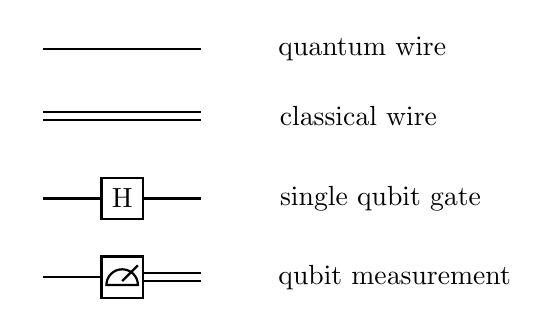
\begin{tikzpicture}[thick]
		
		\tikzstyle{operator} = [draw,fill=white,minimum size=1.5em] 
		
		%\draw (3,3) -- (3,0) ;
		
		\draw (0,3) -- (2,3) ;
		\node at (4.05,3) {quantum wire};
		
		\draw (0,2.1) -- (2,2.1) ;
		\draw (0,2.2) -- (2,2.2) ;
		\node at (4,2.15) {classical wire};
		
		\draw (0,1.1) -- (2,1.1) ;
		\node[operator] (op11) at (1,1.1) {H};
		\node at (4.28,1.1) {single qubit gate};
		
		\draw (0,0.1) -- (1,0.1) ;
		
		\draw (1,0.15) -- (2,0.15) ;
		\draw (1,0.05) -- (2,0.05) ;
		% Define coordinates
		\def\Radius{0.2}
		\path
		(-\Radius, 0) coordinate (A)
		-- coordinate (M)
		(\Radius, 0) coordinate (B)
		(M) +(60:\Radius) coordinate (C)
		+(120:\Radius) coordinate (D)
		;
		
		\node[operator] (op11) at (1,0.1) {};
		\node at (4.46,0.1) {qubit measurement};
		
		% Draw semicircle
		\draw[operator]
		(1.2,0) arc(0:180:\Radius) -- cycle ;
		% Annotations
		
		\draw (1,0.05) -- (1.2,0.25);
		
	\end{tikzpicture}
	\end{figure}	
			
		\bibliography{ref}
		
	\end{document}